\documentclass[standalone]{beamer}

\begin{document}
\section{SMAWK 演算法}

\begin{frame}{\btitle{前言}}
  \begin{itemize}
    \item 前面的轉移點單調,已經讓複雜度從 $O(N^2)$ 的東西壓到 $O(N \log N)$
    \item 現在,要來進一步的壓到 $O(N)$
  \end{itemize}
\end{frame}

\begin{frame}{\btitle{定義}}
  \begin{theorem}
    定義一個 $2 \times 2$ 矩陣 $\begin{bmatrix}
      a & b \\
      c & d
    \end{bmatrix}$ 是單調的,如果以下兩個條件都有成立:

    \begin{itemize}
      \item 如果 $c < d$,那麼 $a < b$
      \item 如果 $c = d$,那麼 $a \leq b$
    \end{itemize}

    而一個 $N \times M$ 的矩陣是 \textbf{完全單調矩陣},若且唯若每個 $2 \times 2$ 的子矩陣(submatrix)都是單調矩陣。注意到子矩陣的列(row),行(column)不一定要是連續的。
  \end{theorem}

  定義 $h(i)$ 是第 $i$ 列中,最左邊最小值發生的位置。而如果 $N \times M$ 的矩陣 $A$ 是一個完全單調矩陣,那麼會有 $h(1) \leq h(2) \leq \dots \leq h(N)$ 這個性質
\end{frame}

\begin{frame}{SMAWK 演算法}
  \begin{itemize}
    \item 而 SMAWK 演算法做的事情,就是給定一個 $N \times M$ 大小的完全單調矩陣,SMAWK 演算法會在 $O(N + M)$ 的時間內,找到 $h(1), h(2), \dots, h(N)$
    \item 這個演算法分成的架構如下:
    \begin{itemize}
      \item 若 $\max(N, M) \leq 2$,暴力算出所有的 $h(i)$。
      \item 若 $N \geq M$,則呼叫 \texttt{interpolate()} 算法,遞迴計算 $\frac{N}{2} \times M$ 矩陣的答案後,找出剩下 $\frac{N}{2}$ 列的答案。
      \item 若 $N < M$,則呼叫 \texttt{reduce()} 算法,把一些不重要的行(column)刪掉後,遞迴呼叫剩下 $N \times N$ 矩陣的答案。
    \end{itemize}
  \end{itemize}
\end{frame}

\begin{frame}{\btitle{interpolate}}
  \begin{itemize}
    \item interpolate 的想法很簡單:把 $N \times M$ 的矩陣分成奇數列與偶數列,把偶數列構成的矩陣拿去遞迴算答案
    \item 當我們有偶數列的答案後,我們就可以根據偶數列的答案,算出奇數列的答案
    \item 根據前面提到的 $h(1) \leq h(2) \leq \dots \leq h(N)$ 的性質,假設我要算奇數列 $h(i)$ 的答案,我們可以發現:$h(i - 1) \leq h(i) \leq h(i + 1)$。也就是說,這個奇數列答案的位置,\textbf{是被前後兩個偶數列的答案位置限制住的}。所以,我們只要跑過 $h(i - 1)$ 到 $h(i + 1)$ 的所有值,就可以知道第 $i$ 行的最小值發生的位置
    \item 也因此,我們就可以花 $O(N + M)$ 加上額外遞迴的時間,完成 interpolate 這個操作。
  \end{itemize}
\end{frame}

\begin{frame}{\btitle{reduce}}
  \begin{itemize}
  \item reduce 這個函數的想法,就是利用矩陣是完全單調的性質,刪掉至少 $M - N$ 個列,讓新的矩陣變成至多 $N \times N$ 後,拿去跑 interpolate
  \item 基本上,會開一個 stack $S$ 來維護要選擇的列。接著,我們會由左而右的看每個列的狀況。假設我們正在看列 $C$,而矩陣的第 $i$ 行第 $j$ 列的值為 $A_{i, j}$。演算法進行過程如下:
  \item 如果 stack 是空的,直接把 $C$ 放進去 stack 裡面。
  \item 否則,執行以下迴圈直到 $S$ 是空的,或者是 $C$ 被擊敗了:
  \begin{itemize}
    \item 假設 stack 裡面有 $x$ 個列,最後一個為 $c_x$。
    \item 如果 $A_{x, c_x} > A_{x, C}$,那麼把 $c_x$ 這列從 stack 中丟掉,因為 $c_x$ 不可能包含最佳解了。
    \item 否則,代表 $C$ 被擊敗了,離開迴圈。
  \end{itemize}
  \item 如果這時候 stack 裡面的列數量小於 $N$ 個,那麼就把 $C$ 丟進 stack 裡面。
\end{itemize}
\end{frame}

\begin{frame}{\btitle{範例}}
  \begin{center}
    \begin{tabular}{|p{0.1\textwidth}|p{0.1\textwidth}|p{0.1\textwidth}|p{0.1\textwidth}|p{0.1\textwidth}|}
      \hline
      10 & 20 & 13 & 19 & 35 \\ [3ex]
      \hline
      20 & 29 & 21 & 25 & 37 \\ [3ex]
      \hline
      28 & 33 & 24 & 28 & 40 \\ [3ex]
      \hline
      42 & 44 & 35 & 38 & 48 \\ [3ex]
      \hline
      48 & 49 & 39 & 42 & 48 \\ [3ex]
      \hline
      56 & 55 & 44 & 44 & 49 \\ [3ex]
      \hline
      75 & 73 & 59 & 57 & 53 \\ [3ex]
      \hline
    \end{tabular}
  \end{center}
\end{frame}

\begin{frame}{\btitle{範例}}
  \begin{center}
    \begin{tabular}{|p{0.1\textwidth}|p{0.1\textwidth}|p{0.1\textwidth}|p{0.1\textwidth}|p{0.1\textwidth}|}
      \hline
       &  &  &  &  \\ [3ex]
      \hline
      20 & 29 & 21 & 25 & 37 \\ [3ex]
      \hline
       &  &  &  &  \\ [3ex]
      \hline
      42 & 44 & 35 & 38 & 48 \\ [3ex]
      \hline
       &  &  &  &  \\ [3ex]
      \hline
      56 & 55 & 44 & 44 & 49 \\ [3ex]
      \hline
       &  &  &  &  \\ [3ex]
      \hline
    \end{tabular}
  \end{center}
\end{frame}

\begin{frame}{\btitle{範例}}
  \begin{center}
    \begin{tabular}{|p{0.1\textwidth}|p{0.1\textwidth}|p{0.1\textwidth}|p{0.1\textwidth}|p{0.1\textwidth}|}
      \hline
       &  &  &  &  \\ [3ex]
      \hline
      \textbf{20} &  & 21 & 25 &  \\ [3ex]
      \hline
       &  &  &  &  \\ [3ex]
      \hline
      42 &  & \textbf{35} & 38 &  \\ [3ex]
      \hline
       &  &  &  &  \\ [3ex]
      \hline
      56 &  & \textbf{44} & 44 &  \\ [3ex]
      \hline
       &  &  &  &  \\ [3ex]
      \hline
    \end{tabular}
  \end{center}
\end{frame}

\begin{frame}{\btitle{範例}}
  \begin{center}
    \begin{tabular}{|p{0.1\textwidth}|p{0.1\textwidth}|p{0.1\textwidth}|p{0.1\textwidth}|p{0.1\textwidth}|}
      \hline
      10 & 20 & 13 & 19 & 35 \\ [3ex]
      \hline
      \textbf{20} & 29 & 21 & 25 & 37 \\ [3ex]
      \hline
      28 & 33 & 24 & 28 & 40 \\ [3ex]
      \hline
      42 & 44 & \textbf{35} & 38 & 48 \\ [3ex]
      \hline
      48 & 49 & 39 & 42 & 48 \\ [3ex]
      \hline
      56 & 55 & \textbf{44} & 44 & 49 \\ [3ex]
      \hline
      75 & 73 & 59 & 57 & 53 \\ [3ex]
      \hline
    \end{tabular}
  \end{center}
\end{frame}


\begin{frame}{\btitle{範例}}
  \begin{center}
    \begin{tabular}{|p{0.1\textwidth}|p{0.1\textwidth}|p{0.1\textwidth}|p{0.1\textwidth}|p{0.1\textwidth}|}
      \hline
      \textbf{10} & 20 & 13 & 19 & 35 \\ [3ex]
      \hline
      \textbf{20} & 29 & 21 & 25 & 37 \\ [3ex]
      \hline
      28 & 33 & \textbf{24} & 28 & 40 \\ [3ex]
      \hline
      42 & 44 & \textbf{35} & 38 & 48 \\ [3ex]
      \hline
      48 & 49 & \textbf{39} & 42 & 48 \\ [3ex]
      \hline
      56 & 55 & \textbf{44} & 44 & 49 \\ [3ex]
      \hline
      75 & 73 & 59 & 57 & \textbf{53} \\ [3ex]
      \hline
    \end{tabular}
  \end{center}
\end{frame}

\begin{frame}{\btitle{時間複雜度}}
  \begin{itemize}
    \item 假設我們拿到一個 $N \times M$ 的矩陣,可以發現大致上需要按照 reduce, interpolate, reduce, interpolate 的順序來執行 SMAWK 演算法
    \item 遞迴式為 $T(N, M) = O(N + M) + T(\frac{N}{2}, N)$
    \item 展開之後可以發現 $T(N, M) = O(M) + 2(O(N) + O(\frac{N}{2}) + O(\frac{N}{4}) + \dots)$,可以發現這是一個 $O(N + M)$ 複雜度的演算法
  \end{itemize}
\end{frame}


\begin{frame}{\btitle{應用}}
  \begin{itemize}
    \item 注意到完全單調矩陣的證明,有的時候要直接證很難。但是,別忘記在前面章節提到的,\textbf{如果那個矩陣符合 monge condition,那麼那個矩陣也會是完全單調矩陣}
    \item 讓我們來看一個例題,底下的例題同時也是 SMAWK 演算法被提出的論文中,論文作者提出來的題目
    \begin{problem}
      給定一個 $N$ 個點的凸多邊形。對於凸多邊形上的每個點 $i$,請求出離點 $i$ 最遠的點的編號。

      % $(N \leq 5 \times 10^5)$
      \begin{itemize}
        \item $N \leq 5 \times 10^5$
      \end{itemize}
    \end{problem}
  \end{itemize}
\end{frame}

\begin{frame}{\btitle{應用}}
    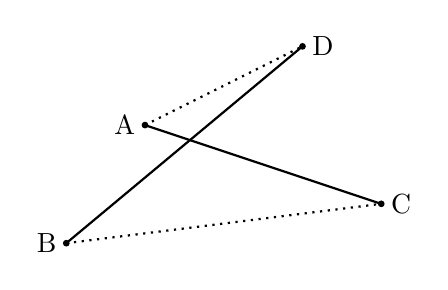
\begin{tikzpicture}[scale=0.5]
\draw[black, thick] (-5, 0) -- (1, 5);
\draw[black, thick] (-3, 3) -- (3, 1);
\draw[black, dotted, thick] (-5, 0) -- (3, 1);
\draw[black, dotted, thick] (-3, 3) -- (1, 5);
\filldraw[black] (-5, 0) circle (2pt) node[anchor=east]{B};
\filldraw[black] (-3, 3) circle (2pt) node[anchor=east]{A};
\filldraw[black] (1, 5) circle (2pt) node[anchor=west]{D};
\filldraw[black] (3, 1) circle (2pt) node[anchor=west]{C};
\end{tikzpicture}

假設 A, B, C, D 這四個點是凸多邊形上按照逆時針順序的四個點。藉由觀察上圖,可以發現 $dis(A, C) + dis(B, D) \geq dis(A, D) + dis(B, C)$。而如果假設那四個點分別是凸多邊形上的第 $x_1, x_2, y_1, y_2$ 個點,就可以把式子寫成 $dis(x_1, y_1) + dis(x_2, y_2) \geq dis(x_2, y_1) + dis(x_1, y_2)$。即可發現這題有「Monge Condition」這個性質
\end{frame}

\end{document}
